% !TeX root = surgery.tex
\section{The Transmission of the Work}
\subsection{The Nepalese Version}

In the present article and the other publications of our research group, we focus on the study 
of what we call the `Nepalese version' of the \SS. The primary rationale behind using this 
designation was outlined in \citet[2--3]{kleb-2021b}, but we consider it necessary to 
reflect upon its meaning here given the conceptual significance that this term occupies in our 
research.
%, given the conceptual significance that this term occupies in our research, we consider it necessary to reflect upon its meaning here.\q{suggestion: but we consider it necessary to reflect upon its meaning here given the conceptual significance that this term occupies in our research.} 
It is possible that in the course of our research, we will refine our understanding of the 
phenomenon and, consequently, review and modify our current interpretation.%\q{is it 
%sufficient to say 'our current interpretation'?}

Put plainly, the `Nepalese version' refers to a hypothetical text-critical reconstruction of the 
wording of the \SS\ that is based primarily on the evidence of three ancient Nepalese 
manuscripts that we have briefly introduced above and that we will describe in more detail in 
a later section.  We call these MSS “Nepalese” not just because they were preserved and 
discovered by modern scholarship 
%to\q{discovered by modern scholarship} the modern scholarship 
in the 
%present-day 
Kathmandu valley
%\q{seeing that you say 'modern scholarship', 'present-day' seems redundant} 
but also because we believe that they were produced in the same area. We conclude this 
because all three MSS are written in a specific variety of Indic scripts which, to the best of our 
knowledge, was not used outside of the region. 

Furthermore, we speak of a single “version” because we hold that these manuscripts
attest to a peculiar line of transmission of the text.  That is to say, in terms of
stemmatic analysis they share %\q{they share [...] while as the same time, bear
% [...]}
a common ancestor or (hyparchetype), while at the same time, they
bear no signs of significant contamination.  This hypothesis was postulated in
\citet{kleb-2010} and reiterated in \citet{kleb-2021a} as the result of a
systematic analysis of two complete chapters (SS.1.3 and SS.1.15) %\q{So far we
% have been using SS.1.3 format}
as well as several shorter excerpts from the \SS\ transmitted in the Nepalese
manuscripts. On the one hand, these studies highlight that all three MSS preserve
a highly uniform text with very few variations, virtually all of which can be
explained as standard scribal errors or corrections. On the other hand,
\citet{kleb-2010,kleb-2021a} systematically compared %systematically compare\q{has
% systematically compared (the subject is singular)}
the concerned textual excerpts with four printed editions, alternative readings
(\dev{pāṭha}s) reported by several commentators, %the \q{several commentators? as
% the list is not exhaustive}commentators (two medieval authors, Cakrapāṇidatta
% and Ḍalhaṇa, as well as an early modern Bengali scholar Haraṇacandra),
parallel passages in other texts, and with a limited number of additional
manuscripts of the \SS. This analysis demonstrated that the text of the \SS\
preserved in the Nepalese MSS differs decidedly from all the above standards of
comparison. In this way, for example, we establish that another Nepalese
manuscript of the \SS, \MS{Kathmandu NAK 1-1146},\footcite{rima-2022} does not
belong to the peculiar line of textual transmission and need not be taken into
consideration when reconstructing the reading of its hyparchetype. 

However, in view of the more than two hundred handwritten copies of the \SS\
preserved in different libraries across South Asia and in the absence of their
systematic inclusion into the project's current collation, the assumption about
the regional character of the transmission line remains hypothetical.\footnote{For
    a list of known manuscript copies of the \SS, see the sources mentioned in
    footnote \ref{SSmss} below.} As a matter of fact, we believe that the Nepalese MSS
    preserve many archaic features of the early \SS\ and it is possible, even likely,
    that some of these features will be found in other manuscripts of this work that
    have yet to be studied.%, particularly in those that contain versions that differ
    % from
    % that propagated by Ḍalhaṇa.
    %As a matter of fact, we believe that the Nepalese MSS preserve many original
    % features of the \SS, and as such, these are likely attested in other textual
    % witnesses as well.\q{I'm not sure of the intended meaning here. Is some contrast
    % intended (i.e., although we believe that [...], many of the same features are
    % likely attested in textual witnesses from other regions as well)?}

Our research group builds upon the above hypothesis about the existence of a 
distinct Nepalese version of the \SS\ and concentrates primarily on the study of 
this text in its own right and, additionally, in comparison to a single version of the 
compendium popularized by its late medieval commentator Ḍalhaṇa and 
recorded in the widely-used \cite{vulgate}.  The present study of 
SS.1.16 also considers the readings found in \cite{acar-1939} and incorporates 
various observations made by both medieval commentators, Cakrapāṇidatta and 
Ḍalhaṇa, into the notes of the edition and some annotations of the translation.
%\q{We also looked at Cakrapāṇi and incorporated his comments into the notes of the edition and some annotations of the translation. Perhaps, here, you means to say, 'builds upon the above hypothesis by a detailed comparison of 1.16 of the Nepalese version with the version popularized by its late medieval commentator Ḍalhaṇa [...]}

The current paper and several earlier publications furnish a large catalogue of
uniform features that are characteristic of the Nepalese MSS and set them apart
from the vulgate version.\footnote{ Earlier publications include, for example,
\cite{hari-2011,wuja-2013,birc-2021,birc-2021a}.} These features of the Nepalese
MSS include orthographic variants, peculiarities in the structure and structuring
elements, as well as the actual wording of the text. As argued elsewhere in this
article, many of these variants are likely to be closer to an archaic version of
the \SS.  This is partly because they preserve a version of the text that appears
to be less edited, that is, slightly more idiosyncratic and original in
expression, that in turn suggests that it precedes later editorial intervention,
according to the principle of \emph{lectio difficilior potior}.
%less understandable,\q{[...], that is, a less easily understood, [...]}
%version of the text, and thus invoke the principle \emph{lectio difficilior
%    potior}.\q{I'm not too sure of the meaning of the last phrase. Is 'invoking this
%    principle' a reason for these  variants being likely closer to the original? Maybe
%    you mean something like, [...] text, which suggests it was closer to the original
%    according to the principle of \emph{lectio difficilior potior}.}
%
%We\q{I'd drop the  'not just because' in the previous sentence. If you retain it, you need 
%something at the beginning of the next sentence to link to it, such as [not just
% because ...]. On
%the contrary [...]. Both reasons are important, so you could just say,'many of
% these variants
%are likely to be closer to the original for two reasons. Firstly, [...]. Secondly
% and
 % 
We also assign a high historical value to many Nepalese readings  because they
constitute an internally more consistent and coherent text that is at times
further supported by external testimonia.

Additionally, we want to make it clear that we do not think that the Nepalese MSS
provide a so-called original text of the \SS.  Rather, the Nepalese MSS are
witnesses to a hyparchetype, not the archetype, of the \SS.  The Nepalese MSS
provide us with an intermediary node in the history of this work between the
oldest reconstructable text and the vulgate version that was known to Ḍalhaṇa in
the twelfth century and is reproduced in printed editions of the \SS.  The oldest
reconstructable text will only come into focus when all surviving witnesses for
the work are studied.  Having said that, our belief is that the Nepalese version
is certain to be closer to the oldest reconstructable text than are contemporary
printed versions of the work. One of the reasons for this belief is simply that
the Nepalese MSS give us physical evidence for the state of the work in the ninth
century, which cannot be many centuries later than the original assembly of the
work in the form we are familiar with, i.e., a work of five topical sections with
a large added sixth section, the Uttaratantra, that has a somewhat different
character. 
%, on surgery, the expulsion of demons that attack
%children, and disease aetiologies and therapies.

%In editing the Nepalese version, we occasionally make use of corrections and
% emendations,
%and, as far as the reconstructed text is concerned, we believe that it
%
%bears signs of secondary editorial effort.\q{This is not clear. I think you mean
%    to say that the Nepalese mss attest to a hyparchetype rather than the
% archetype of
%    the \SS. Our use of emendations and corrections is not proof of this, because
%    these methods are needed whether we are constructing an archetype or
% hyparchetype.
%    Signs of past redactors editing the text is possible proof (and do you have
% refs
%    or examples?) but such signs might also be the result of an author's attempt
% to
%    compile older materials. The point you make below about the colophons strikes
% me
%    as more of a scribal issue rather than authorial one.} 
% Nevertheless, we think that
%

To summarize: the evidence arising from our studies to this point leads us to think that the
Nepalese MSS provide access to single line of textual transmission that goes back
to a hyparchetype that predates the composition of all major commentaries on the
\SS\ and that, due to its regional character, has suffered relatively little
contamination. We term this hyparchetype the “Nepalese version.” 
%When evaluating
% these
% readings historically, it is further necessary to keep in mind that there is
% plentiful evidence suggesting an ancient age of the readings accepted into
% Ḍalhaṇa’s version of the text.


\subsection{The Versions of Cakrapāṇidatta and Ḍalhaṇa}

The commentaries of Cakrapāṇidatta and Ḍalhaṇa, titled \emph{Bhānumatī} and
\emph{Nibandhasaṅgraha} respectively, are based on similar but not identical
versions of the \SS, both of which are significantly different to the Nepalese
version.\footnote{See \cite[IA 374--379]{meul-hist} on these authors. Meulenbeld
already noted that “the text of the \SS\ in the [1939] edition of the
\emph{Bhānumatī} differs at many places from the text of the [vulgate edition of
1938]” and gave examples from the \emph{sūtrasthāna} \citep[IB, 496, note
76]{meul-hist}.} Ḍalhaṇa was aware of Cakrapāṇidatta's work and reiterated many of
his predecessor's remarks, so the interpretation of the root text by these two
commentators is, broadly speaking, consistent.\footcite[IB, 499,
n.\,162]{meul-hist}  Ḍalhaṇa evidently also had several manuscripts of the \SS\
available to him, since he frequently recorded their variant
readings.\footnote{Cf.\ \cite[IA, 377]{meul-hist}.  Meulenbeld drew attention to
Ḍalhaṇa's commentary on \Su{5.8.24cd--25ab}{587} as a particularly striking
example of such awareness \citep[IB, 497, n.\,112]{meul-hist}.  In this passage, Ḍalhaṇa
noted that certain readings known to the earlier commentators Jejjaṭa and Gayadāsa
were, “not to be found in current manuscripts” (\dev{sa ca vartamānapustakeṣu na
dṛśyate}).}

In addition to the fine-grained issues raised by the relationship between these
commentators, there are added difficulties introduced by the way the editors of
the printed versions of these commentaries handled the texts in several cases. The
most obvious difficulty is that \citeauthor{acar-1939}'s text of the
\emph{Sūtrasthāna} commented on by Cakrapāṇidatta \citep{acar-1939} simply
duplicated the text of that section from \citeauthor{vulgate}'s edition of
Ḍalhaṇa's commentary \citep{vulgate}.\footnote{There are a few exceptions where
Cakrapāṇidatta glossed a word or compound that is different to the one glossed by
Ḍalhaṇa. For example, in SS.1.16.18, Cakrapāṇidatta glossed \dev{rājasarṣapa}
whereas Ḍalhaṇa glossed \dev{gaurasarṣapa}, and the editors reflected this in the
root texts of the \emph{Bhānumatī} \citep[130]{acar-1939} and
\emph{Nibandhasaṅgraha} \citep[79]{vulgate} respectively.} This duplication of the
root text creates the misleading impression that both commentators had the same
\SS\ before them. However, there is much evidence, including in SS.1.16, that this
was not the case. For example, Ḍalhaṇa commented on four verses,
\Su{1.16.11–-14}{78}, as part of his root text, that Cakrapāṇidatta cited
separately only in his commentary \citep[128–129]{acar-1939}.  Cakrapāṇidatta
introduced each verse with “some people say” (\dev{kecit paṭhanti}). This clearly
indicates that these verses were not in the version of the \SS\ upon which
Cakrapāṇidatta was commenting, but a century or so later they were part of the
text before Ḍalhaṇa.  But \citeauthor{acar-1939} included them in the root text
of the \SS\ as if they were.  Such cases make it harder than it would otherwise be
to remain clear that these two commentators were working off different versions of
the \SS.

Also, Cakrapāṇidatta did not acknowledge or comment on some verses in the version
of the \SS\ known to Ḍalhaṇa. Although it is possible that a commentator may not
have remarked on a verse because its meaning was clear, in some cases the
commentarial convention of citing the first words of a new verse or passage
provides firmer ground for suspecting the absence of a verse in the root text. 

To give an example, there is a prose passage at Su.1.16.18 of the \SS\ that
Cakrapāṇidatta commented on in his
\emph{Bhānumatī} (Fig.\,\ref{fig:yavasva}, left).\footnote{\cite[130]{acar-1939}, i.e.,
\dev{athāpraduṣtasyābhivardhanārtham \ldots\ nidadhyāt/}. It is numbered
Su.1.16.19 in Dalhaṇa's \emph{Nibandhasaṅgraha} \citep[79]{vulgate}.} It is
followed by several verses also in the main text  of the \SS\ that elaborate on
the content of the prose passage.\footnote{Su.1.16.19--23 in \cite{acar-1939},
i.e., \dev{svedito \ldots}, \dev{yavāśva \ldots}, \dev{tailaṃ \ldots}, \dev{teṣām
\ldots}, \dev{vaddha \ldots}.} 
%\q{You say, “Both Cakrapāṇidatta and Ḍalhaṇa
%    introduced these verses and cited the opening words of the first verse before
%    glossing specific terms.” but that's not right. Bhānumatī shows no awareness of
%    verses 19-21ab.  Cakra doesn't say “svedito...”.}\q{Took out: ”Cakrapāṇidatta
%    did not introduce, cite or comment on the same verses as Ḍalhaṇa
%    (Su.1.16.20--22ab, \cite[79]{vulgate}).”} %Although
% these
% verses are discussed by Ḍalhaṇa appears in the root text of
%\citeauthor{acar-1939}'s
%edition of the \emph{Bhānumatī} (Su.1.16.19, \cite[130]{acar-1939}), and the
%others (SS.1.16.20--21ab) are included in that edition in parenthesis
%
%although the
%editors note in a footnote that the verses did not appear in Nepalese manuscript
%they consulted.
Ḍalhaṇa commented on these explanatory verses (Fig.\,\ref{fig:yavasva}, right), 
\begin{figure}[t]
    \centering
    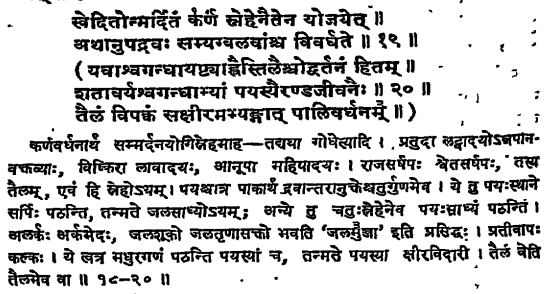
\includegraphics[width=.58\textwidth]{media/yavasva-cakra}\
    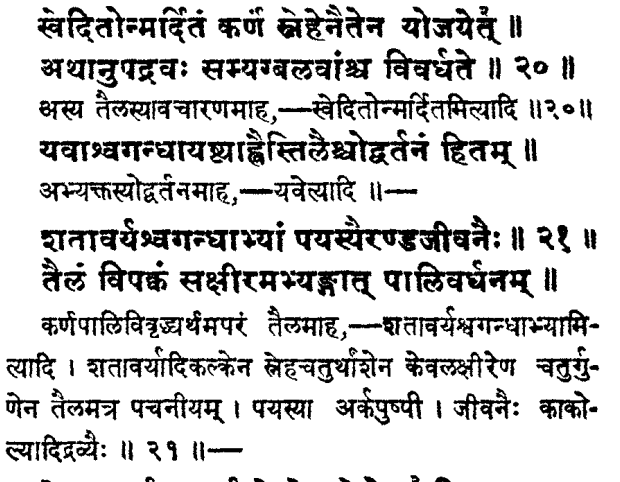
\includegraphics[width=.41\textwidth]{media/yavasva-dalhana}
    \caption{The text as it appears in Cakrapāṇi (left) and Ḍalhaṇa (right)  
    (\cite[130]{acar-1939}, \cite[79]{vulgate}).}
    \label{fig:yavasva}
\end{figure}
citing keywords that show they all
formed part of the main text of the \SS\ that was before
him.\footnote{\Su{1.16.19--23}{79--80}.} However, Cakrapāṇidatta's older
commentary showed no awareness of the first few verses in this group,
Su.1.16.19--21ab.\footcite[130--131]{acar-1939}  Apparently, they were not part of
the text of the \SS\ as he knew it.  In spite of that, the editors printed these
verses in their edition of Cakrapāṇidatta's work as if they were indeed part of
the \SS\ known to to him.\footnote{The editors remarked in a footnote that verses
20--21a were not in the Nepalese manuscript that they consulted \citep[130,
n.\,2]{acar-1939}.}

A similar instance of this occurs in the edition of the \emph{Bhānumatī} at \SS\,1.16.31 
\begin{figure}[t]
    \centering
    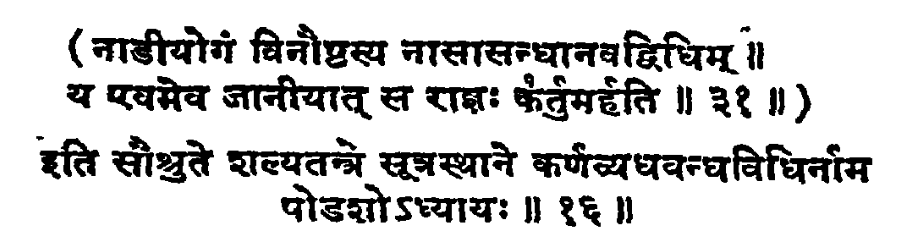
\includegraphics[width=.75\linewidth]{media/nadiyogam}
    \caption{\SS\,1.16.31 in the 1939 printed edition.}
    \label{fig:nadiyogam}
\end{figure}
where the editors of the 1939 printed edition included a verse in parenthesis that was
commented on by Ḍalhaṇa but not by Cakrapāṇidatta (see 
Fig.\,\ref{fig:nadiyogam}).\footnote{The verse begins 
\dev{nāḍīyogaṃ vinauṣthasya}.  It is printed in the vulgate as 
\Su{1.16.32}{81}, with Ḍalhaṇa's commentary.  It is printed in parentheses as 1.16.31 in the 
edition of the Bhānumatī \citep[133]{acar-1939}.} This verse was almost certainly not in the 
text of the \SS\ known to Cakrapāṇidatta. 



The manuscript on which the editor's edition of the \emph{Bhānumatī} was
mainly based,  \MScite{London BL H. T. Colebrooke 908}, does not include the root text of 
the \SS.\footnote{% 
% DW: we don't need to depend on Eggeling because we've now got the MS.
%This observation is based on the
%opening passage \MScite{London IOLR 908}.  
The MS is described in \cite[vol.\,1.5, 928, \#2647]{egge-1887}. 
%of MS 1887-1935 of the \emph{Bhānumatī},
% which is transcribed in Eggling 1896: 928.
%The transcription in this catalogue also shows the commentary without the root text. 
The section on p.\,\pageref{1939edition} below describes the sources that the editors used 
for the 1939 edition.}  Therefore, it requires a detailed reading  of the commentary itself to 
infer what its author, Cakrapāṇidatta, was seeing in the manuscripts of the \SS\ that he had 
before him in the eleventh century.  But, to summarize, there is no evidence that they  
included the verses SS.1.16.19–-21ab and 31 that are printed in \cite{acar-1939} as if they 
were present to Cakrapāṇidatta. 

% got to here

% Ḍalhaṇa 1.16.11–14
%The version of 1.16.11–14 known to Ḍalhaṇa \citep[78]{vulgate} has four verses (\emph{śloka}) at this point that are not in the Nepalese manuscripts. The additional verses iterate the types of joins required for ear flaps that are missing, elongated, thick, wide, etc. All four verses were probably absent in the version of the \emph{Suśrutasaṃhitā} known to Cakrapāṇidatta. He cites the verses separately in his commentary, the \emph{Bhānumatī} \citep[128–129]{acar-1939}, introducing each one as 'some people read' (\emph{ke cit paṭhanti}). However,  in Trikamajī Ācārya's edition of the \emph{Sūtrasthāna} of the \emph{Bhānumatī}, the root text is largely identical to the one commented on by Ḍalhaṇa (\cite{vulgate}), even in instances like this where Cakrapāṇidatta's commentary indicates that he was reading a different version of the \emph{Suśrutasaṃhitā}

% Ḍalhaṇa 1.16.19–20 
%Cakrapāṇidatta \citep[131]{acar-1939} does not comment on these verses, nor verse 15 of the Nepalese version, and so the version of the \emph{Suśrutasaṃhitā} known to him may not have included them.

% Ḍalhaṇa 1.16.32
 %Cakrapāṇidatta \citep[133]{acar-1939} does not comment on this additional verse, which suggests that either he did not know of it or was not inclined to accept it.
 
% Both commentators were aware of a version of the \SS\ that was similar to the Nepalese version % See blog.
\subsubsection{Cakrapāṇidatta and the Nepalese version}
In fact, there is some evidence that the Nepalese version of the \SS\ was more
similar to Cakrapāṇidatta's version than to Ḍalhaṇa's. For example, \SS\,1.16.5 of
the Nepalese version begins with the compound
\dev{doṣasamudayāt}.\footcite[126]{acar-1939} Ḍalhaṇa's version, on the other
hand,  inserted two compounds, \dev{kliṣṭajihmāpraśastasūcīvyadhāt} and
\dev{gāḍhataravartitvāt}, before this.\footnote{\SS\ \Su{1.16.6}{77}.} Cakrapāṇidatta
began his comment on this passage by glossing \dev{doṣasamudayāt}, which
suggests that he was not aware of the compounds that Ḍalhaṇa
saw.\footnote{\SS\,1.16.5 \citep[126–127]{acar-1939}.}

If one looks beyond \SS\,1.16, there are instances where the Nepalese version and
the root text as read by Cakrapāṇidatta have the same reading, but Ḍalhaṇa
mentions it as an alternative that is, “read by others.” For example, \SS\,1.1.28 of
the Nepalese version has \dev{tatrāsmiñ chāstre}, which is also the reading
commented on by Cakrapāṇidatta.\footcite[17]{acar-1939} However, Ḍalhaṇa comments
on \dev{asmiñ chāstre} and states that “others read \dev{tatrāsmiñ
    chāstre}”.\footnote{\SS\ \Su{1.1.22}{5}.} %Also, in his commentary on SS.1.1.8.1,
%Ḍalhaṇa notes the variant reading \dev{ṣaṣṭyā vidhānaiḥ}, which is not in his
% root
%text but evidently was in Cakrapāṇidatta's.\footnote{See \Su{1.1.8.1}{5} and
%SS.1.1.6 \citep[11]{acar-1939} respectively.}
Another example is the reading of \dev{ṣaṣṭyā vidhānaiḥ} in Ḍalhaṇa's commentary
on \Su{1.1.8.1}{3} that is not in his main text but that he ascribes to “some
others.” This reading is likely to be derived  from the expression
\dev{ṣaṣṭyābhidhānaiḥ} in the main text of the Nepalese version, and to have been 
rewritten before Ḍalhaṇa's time because it was hard to understand.\footnote{See
the discussion by \citet[4--5]{birc-2021a}.}

% Ḍalhaṇa was aware of the reading in the Nepalese version because he notes in his commentary on 1.16.6 \citep[77]{vulgate} that some read 'because of the accummulation of humours' rather than 'because of piercing with a painful, crooked and unrecommended needle or because of a wick that is too thick.' 

\subsection{Differences between the Nepalese and Subsequent Versions of SS.1.16}

% The structural differences between the Nepalese and subsequent versions has been 
%discussed by \citet[27–44]{kleb-2021b}, which include the frame story,\footnote{On this 
%topic, also see the more recent \citet{birc-2021}.} the name of the first book 
%(\emph{Ślokasthāna}), the structuring of the text according to chapter and section 
%colophons, 
%and an additional passage in the \emph{Kalpasthāna}. \citet[44–55]{kleb-2021b} also 
%makes 
%general observations on distinct features of the Nepalese version's content and looks 
%specifically at lists of skin lesions arising from urinary disease and vital energies. And in an 
%effort to demonstrate the possibility of greater coherence in the Nepalese version, 
%\citet[101–104]{hari-2011} has compared its classification of snakes with Ḍalhaṇa's 
%version. 

% On the whole, these observations indicate that [...synopsis of general conclusions here, Andrey?...]
%% 1.16 is missing yathovāca bhagavān dhanvantariḥ|

Several differences between the text of the \SS\ as found in its multiple printed
versions and as reconstructed on the basis of the Nepalese MSS have already been
pointed out in previous publications.  \citet[27\,f]{kleb-2021b} listed
differences in the chapter sequence as they affect the overall organization and
structuring themes and elements of the text.  Others have explored variations in
the frame story of the work as a whole.\footcites {wuja-2013} [28-32]{kleb-2021b}
{birc-2021} [2-4]{birc-2021a} \citeauthor{kleb-2021b} highlighted the
interchangeable use of two names of the first book of the text, namely
\emph{Ślokasthāna} and \emph{Sūtrasthāna}. He also discussed another peculiarity
of the Nepalese version, namely the additional verse or prose colophons found at
the end of each book and also at the end of each decade of chapters of the
work.\footcite[32--44]{kleb-2021b}

As the present paper demonstrates, many distinct features pertaining to the actual
content of the Nepalese version continuously come to light as we proceed with our
study of the manuscripts. 

\citet[101–104]{hari-2011} provided an exemplary investigation of textual variants in the 
Nepalese version.  His study looked at the classification of snakes in
\SS\,5.4 and revealed that the Nepalese MSS preserve a text that is internally
more consistent and coherent than the versions of the \SS\ found
in different printed sources.

Klebanov too has contributed some general remarks and examples of substantive differences 
between the Nepalese and vulgate texts 
and detailed two particular case studies.\footcite[44--55]{kleb-2021b} The first
case study dealt with the list of skin lesions associated with urinary disease
(\dev{pramehapiṭakā} in the Nepalese spelling).  Their signs and pathogenesis are
described in the Nidānasthāna and their treatment in the 
\emph{cikitsāsthāna}.\footnote{\Su{2.6}{289--294} and 
\Su{4.12}{454--455} respectively.} 
This list of skin lesions exemplifies a case where the text of the \SS\ transmitted
in the Nepalese MSS is internally more coherent than that commented on by Ḍalhaṇa.
The incoherence of Ḍalhaṇa's version was already identified by an earlier
commentator, Gayadāsa (fl.\,ca.\,1000), 
who
proposed a textual conjecture that corresponds to the reading of the Nepalese
version.\footnote{\MScite{Kathmandu KL 699} was copied a century or more before
    Gayadāsa's time, so its version cannot have been influenced by Gayadāsa's
    innovations or suggestions.} 

The second case study by \citet{kleb-2021b} focussed on the variation in another
list, that of the bodily winds (\dev{prāṇa}s, \SS\ 3.4).
This  discussion  too relied upon Gayadāsa's learned remarks. 
He commented on a version of the \SS\ corresponding to the Nepalese MSS 
and reported an alternative reading and its interpretation preferred
by another ancient commentator, Jejjaṭa.  It is precisely 
Jejjaṭa's reading that is known to modern
readers of the \SS\ from the vulgate version of the text. 

The present paper also provides an example of
interpolation.  This is a rare case in which we have a fairly good idea of where
the inserted text came from, namely the medical theory associated with the
\emph{Carakasaṃhitā}.

% got to here. 2022-09-08

On the whole, these observations indicate that many features of the Nepalese version of the 
\SS\ are likely to go back to an early state of the work that was common to other versions of 
the compendium. 
However, other textual features, such as the text-structuring colophons concluding every 
tenth chapter, are likely to have occurred within a local Nepalese transmission of the text, 
and it is improbable that they are attested in the MSS from other regions. 
When evaluating the Nepalese readings historically, it is necessary to keep in mind that there 
is plentiful evidence that Ḍalhaṇa's version of the text also included extremely early 
readings and variants, suggesting that some of the readings accepted by Ḍalhaṇa were 
ancient, if not original.  Each case has to be weighed. 


The following detailed comparison of 1.16 of the Nepalese version with Ḍalhaṇa's 
\emph{Nibandhasaṅgraha} unfolded as the chapter was edited. The differences appear to 
emanate largely from attempts to standardise, simplify or clarify the language of the 
Nepalese version, add and redact information, and introduce changes to recipes and 
treatments. Examples from 1.16 have been provided to demonstrate the general 
observations which, it is hoped, a larger survey of the text will support.

Table \ref{fig:chapters} reveals the extent to which 1.16 of the Nepalese version
was redacted to create the one known by Ḍalhaṇa. In this particular case,
twenty-seven verses have been added.  Eight of these verses (11--14, 21--22ab,
23cd--24, 32) are well-integrated with the existing material in so far as they
reiterate and elaborate on the content of passages in the Nepalese version. A
block of nineteen verses (26.1--19) at the end of this chapter in Ācārya's edition
of the \emph{Nibandhasaṅgraha} (\cite[80]{vulgate}) was known by Ḍalhaṇa. These
verses cover additional diseases of the ear lobes, with their treatment and
complications. Although Ḍalhaṇa conceded that some read them in this chapter, he
concludes that they were not composed by sages and, therefore, should not be read.
Ācārya probably included these verses because they were in his manuscripts,and
Ḍalhaṇa's comments prompted him to place them in parentheses.\footnote{Ācārya
    (\cite[80]{vulgate}) did not state that these verses were absent in some or all of
    his manuscripts, which he usually did in a footnote if this was the case. A
    broader survey of manuscripts would be helpful for establishing whether these
    verses were part of the transmission of the \SS\ in India. For example, they are
    present in \MScite{Hyderabad Osmania 137-3(b)}.}  Be this as it may, this large
    block of verses is absent in the Nepalese version.  
\begin{figure}[t]
\centering
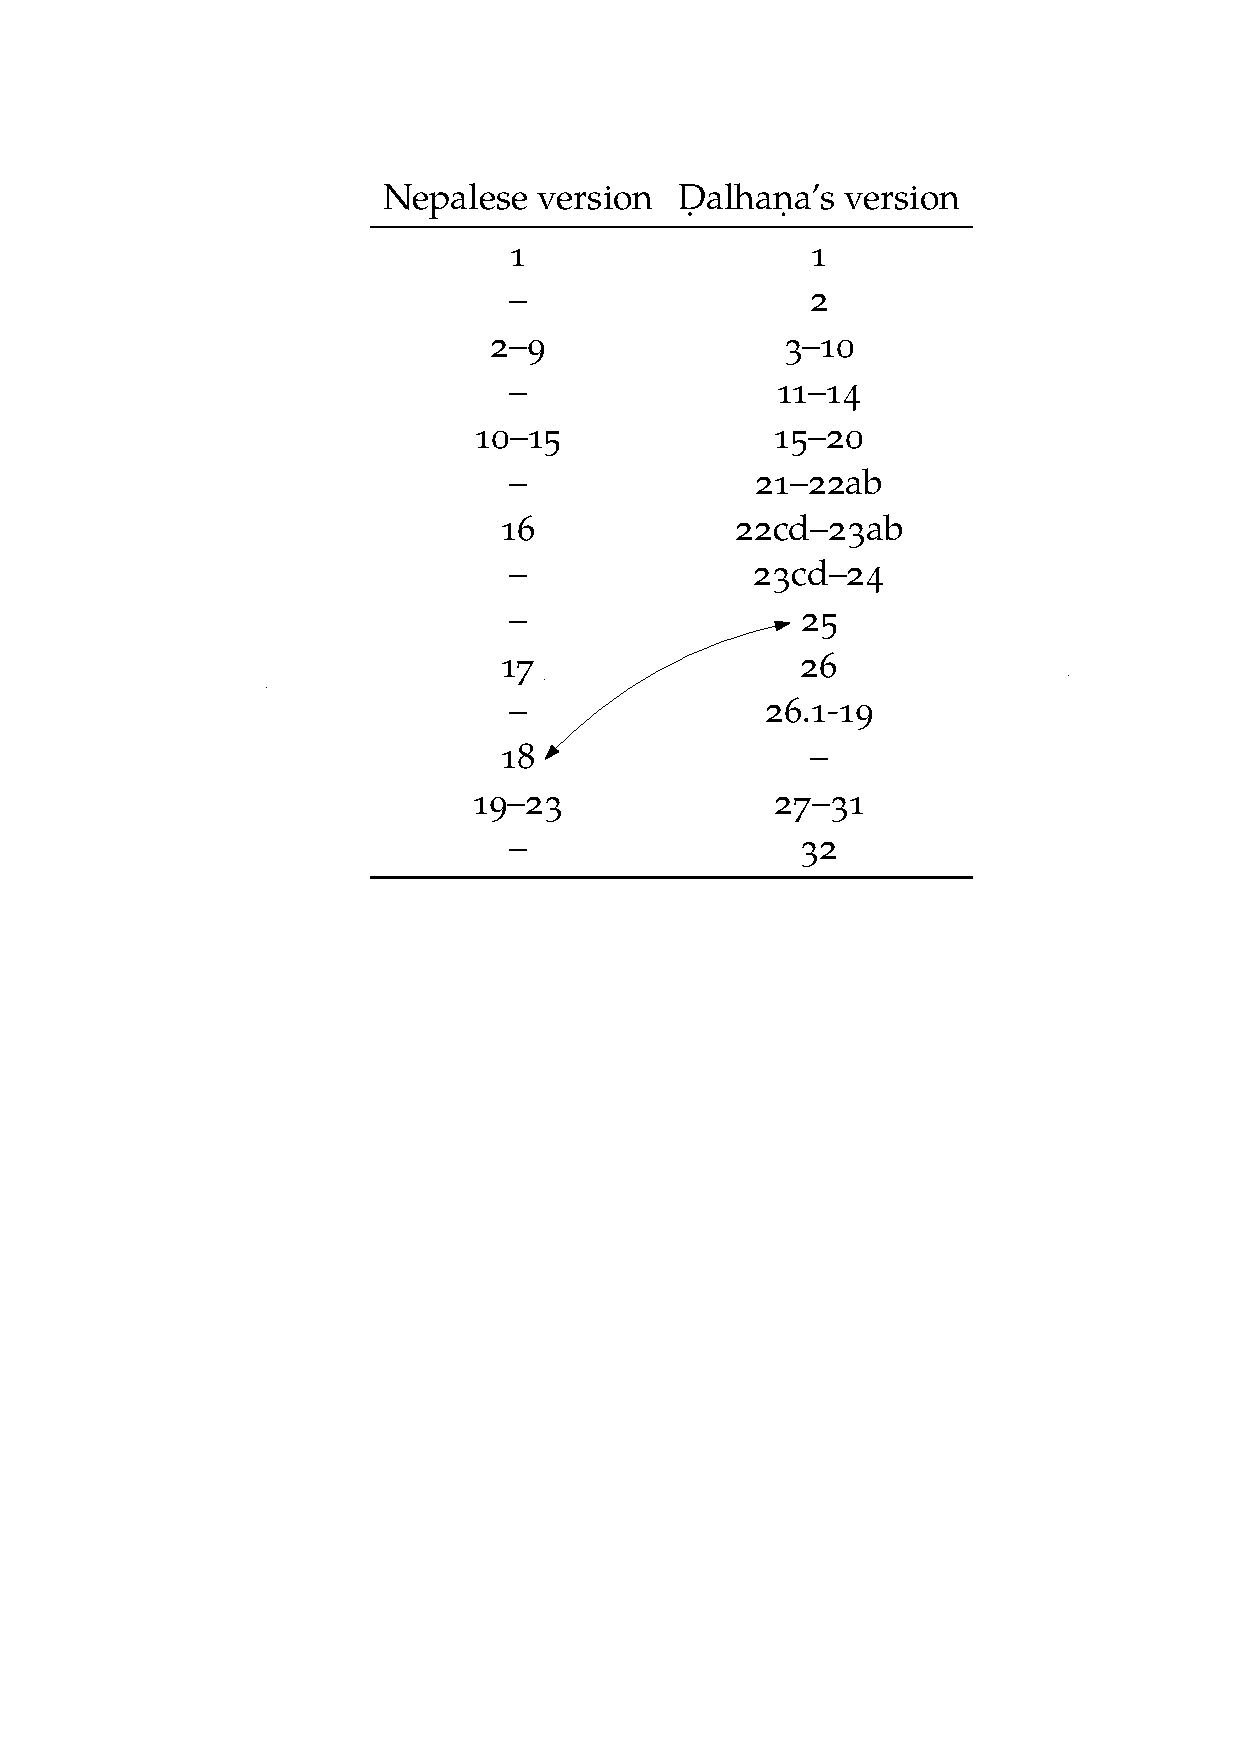
\includegraphics[draft=false,width=.75\textwidth]{table-of-versions.pdf}
\caption{A Comparison of verses in 1.16 of the Nepalese and Ḍalhaṇa's versions.}
\label{fig:chapters}
\end{figure}

In Table \ref{fig:chapters}, one can also see that verses 17 and 18 of the
Nepalese version were transposed in the redaction of Ḍalhaṇa's version, in which
they are numbered 26 and 25 respectively. Although this only occurs once in 1.16,
such transposing of verses and even their hemistiches is common in the
redaction of other chapters of the \SS.

Apart from the addition of verses, the redacting of the version known to Ḍalhaṇa involved 
many small, yet sometimes significant, changes that are summarised below.\footnote{The 
present study focusses on the commentary of Ḍalhaṇa, but many of the same investigations
    could be made with regard to the surviving parts of the other early commentaries. See the 
    discussion below, p.\,\pageref{ref:dalhana}.}

\subsubsection{Changing Spelling, Sandhi and Syntax}


Later commentators like Ḍalhaṇa often made efforts to standardise, simplify or improve 
the language of the Nepalese version. Such changes include the standardising of 
spelling,\footnote{For example, \dev{pattāṅga} (SS.1.16.21) → \dev{pataṅga} (1.16.29, 
\cite[81]{vulgate}). For more information on this, see the relevant footnote to the 
translation.} sandhi,\footnote{or example, \dev{°hastena ṛju} (SS.1.16.2) → 
\dev{°hastena rju} (1.16.3, \cite[76]{vulgate}).} and verbal forms,\footnote{For example, 
\dev{unnāmayitvā} (SS.1.16.21) → \dev{prānnamya} (1.16.29, \cite[81]{vulgate}); 
\dev{avacūrṇayīta} (SS.1.16.21) → \dev{upaharet} (1.16.29, \cite[81]{vulgate}).} as well 
as interventions to simplify and clarify syntax.\footnote{For example, 
\dev{śoṇitabahutvanivedanāyāṃ cānyadeśaviddham iti jānīyāt | nirupadravatā 
taddeśaviddhaliṅgam |} (SS.1.16.3) → \dev{śoṇitabahutvena vedanayā cānyadeśaviddham 
iti jānīyāt | nirupadravatayā taddeśaviddham iti |} (1.16.4, \cite[76]{vulgate}); 
\dev{āmatailapariṣekeṇopacaret} (SS.1.16.6) → \dev{āmatailena pariṣecayet} (1.16.7, 
\cite[77]{vulgate}); \dev{suparigṛhītaṃ} (SS.1.16.10) → \dev{suparigṛhītaṃ ca kṛtvā} 
(1.16.15, \cite[78]{vulgate}); \dev{anena} (SS.1.16.15) → \dev{snehenaitena} (1.16.20, 
\cite[79]{vulgate}).} These efforts often involved splitting compounds.\footnote{For 
example, 
\dev{yadṛcchāviddhāyāṃ sirāyām} (SS.1.16.4) → \dev{yadṛcchayā viddhāsu sirāsu} 
(1.16.5, \cite[76]{vulgate}); \dev{dhānyāmlakapālacūrṇaṃ} (SS.1.16.10) → 
\dev{dhānyāmlaṃ kapālacūrṇaṃ} (1.16.20, \cite[78]{vulgate}).} In some instances, these 
changes improved the grammar,\footnote{For example, \dev{surāmaṇḍakṣīram} 
(SS.1.16.10) → \dev{surāmaṇḍaṃ kṣīram} (1.16.15, \cite[78]{vulgate}).} or altered the 
meaning.\footnote{For example, \dev{kṣīṇālpamāṃsaḥ} (SS.1.16.12) → \dev{kṣīṇo 
'lpamāṃsaḥ} (1.16.17, \cite[79]{vulgate}).} However, some prefixes of verbal 
forms,\footnote{For example, \dev{samvarddhitaḥ} (SS.1.16.8) → \dev{vivarddhitaḥ} 
(1.16.9, \cite[77]{vulgate}); \dev{niveśya} (SS.1.16.10) → \dev{sanniveśya} (1.16.15, 
\cite[78]{vulgate}); \dev{avabadhya} (SS.1.16.10) → \dev{ca baddhvā} (1.16.15, 
\cite[78]{vulgate}).} case endings,\footnote{For example, \dev{māse} (SS.1.16.2) → 
\dev{māsi} (1.16.3, \cite[76]{vulgate}).} and indeclinables were changed for less apparent 
reasons.\footnote{For example, \dev{api} (SS.1.16.13) → \dev{vā} (1.16.18, 
\cite[79]{vulgate}); \dev{ca} (SS.1.16.16) → \dev{tu} (1.16.23, \cite[79]{vulgate}); 
\dev{tu} (SS.1.16.18) → \dev{ca} (1.16.25, \cite[80]{vulgate}).} There is also a tendency 
to replace uncommon words with generic ones,\footnote{For example, \dev{mrakṣayet} 
(SS.1.16.15) → \dev{yojayet} (1.16.20, \cite[79]{vulgate}); \dev{nahyet} (SS.1.16.21) → 
\dev{baddhvā} (1.16.29, \cite[81]{vulgate}).} add indeclinables,\footnote{For example, 
[absent]  (SS.1.16.6) → \dev{ca} (1.16.7, \cite[77]{vulgate}); [absent] (SS.1.16.10) → 
\dev{tatra} (1.16.15, \cite[78]{vulgate}); [absent]  (SS.1.16.12) → \dev{api} (1.16.17, 
\cite[79]{vulgate}).} omit the verb to be at the end of sentences,\footnote{The words 
\dev{bhavati} or \dev{bhavanti} are omitted four times in Ḍalhaṇa's version (1.16.10 
(twice), 1.16.17 and 1.16.18, \cite[77, 79]{vulgate}).}and introduce verses after a prose 
passage with the phrase \dev{bhavati cātra}.\footnote{For example, [absent] (SS.1.16.11) 
→ \dev{bhavati cātra} (1.16.16, \cite[79]{vulgate}).} 

% Spelling
% 9. nemī → nemi
% 9. yaṣṭī → yaṣṭi
% 9. kākauṣṭhaḥ → kākauṣṭhakaḥ
% 21. pattāṅga → pataṅga *

%Sandhi
% 2 °hastena ṛju  →  °hastena rju (standardise)*

% Standardising and Simplifying Syntax
% 3.  śoṇitabahutvanivedanāyāṃ cānyadeśaviddham iti jānīyāt | nirupadravatā taddeśaviddhaliṅgam || → śoṇitabahutvena vedanayā cānyadeśaviddham iti jānīyāt || nirupadravatayā taddeśaviddham iti ||*
% 6 āmatailapariṣekeṇopacaret → āmatailena pariṣecayet*

% Clarifying syntax
%15 anena → snehenaitena*

% Splitting compounds
% 4. yadṛcchāviddhāyāṃ	sirāyām	 → 	yadṛcchayā viddhāsu	sirāsu (clarifies syntax)*
% 10. surāmaṇḍakṣīram → surāmaṇḍaṃ kṣīram (improves grammar)*
% 10. dhānyāmlakapālacūrṇañ → dhānyāmlaṃ kapālacūrṇañ*
% 12. kṣīṇālpamāṃsaḥ → kṣīṇo 'lpamāṃsaḥ (changes the meaning)*

% Changing verbs and gerunds
% 2. vyadhayet → vidhyete (perhaps, picking up on karnau)
% 6. kurvīta → dadyāt (middle to active) 
% 7. muñcet → kuryāt
% 9. bandhyā bhavanti → sādhyāḥ
% 10. suparigṛhītaṃ → suparigṛhītaṃ ca kṛtvā ( attempt to improve syntax)*
% 10. upapādya → upadhārya
% 10. sandarśya → sandadhyāt | tato (attempt to simplify the sentence)
% 13. chidyeta → chidyate (opt to pres)
% 15. mrakṣayet → yojayet * (replacing less common words with generic ones)
% 21. nahyet → baddhvā*
% 21. unnāmayitvā → prānnamya (standardise)*
%21 avacūrṇayīta → avacūrṇayet (standardise)*

% Omitting bhavati
% Happens a few times; e.g., 1.16.9 (twice), 1.16.12, 1.16.13

% Changing Prefixes
% 8. samvarddhitaḥ → vivarddhitaḥ*
% 10. niveśya → sanniveśya*
% 10. avabadhya → ca baddhvā*
% 15. marditaṃ → unmarditaṃ*
% 21. unnāmayitvā → prānnamya *

% Changing case endings
% 2. māse → māsi (shift from māsa to mās. Can't see a reason)
% 3. śoṇitabahutvanivedanāyāṃ →  śoṇitabahutvena vedanayā (splitting compounds, but locative of circumstance or condition changed to instrumental of reason. latter is clearer, but not much in it)
% 19. viśleṣitāyām atha nāsikāyāṃ → °tāyās tv nāsikāyāḥ

% changing indeclinables
%13 anyathā → ato 'nyathā
% 13 api → vā*
% 15 tataḥ → ataḥ
% 16 ca → tu*
% 18 tu → ca*
% 19 atha → tu
% 23 vai → syāt

% Adding indeclinables
% 10 [absent] → tatra
% 6 [absent] → ca
% 9 [absent] → tu
% 10 [absent] → ca
% 12 [absent] → api
% 14 [absent] → vā

% Omitting indeclinables
% 9 tatra → [absent]
% 9 ca → [absent]

%Adding bhavati cātra before verses.

% Not sure
% 2
% kṛtamaṅgalaṃ svastivācanan → kṛtamaṅgalasvastivācanan (the latter makes better sense, but could have been original, in my opinion, or an attempt to better integrate a gloss that had become part of the text.)
% abhisāntvayamānaḥ → abhisāntvayan (shift from Pres Pass Part to Pres Act Part) % It seems only the latter is correct in the given context. So, it could be just an error in the NV. Emend or Change translation!!! 
% % 10. agropaharaṇīyāt appears to be an error in the NV that needs to be emended.

\subsubsection{Changing Technical Terms}

There is evidence of standardising and altering technical terminology in versions
of the \SS\ subsequent the Nepalese one. Two examples of this in \SS\,1.16 are the
terms for \se{bandha}{joins} and \se{vadhra}{a slice of flesh}. The Nepalese
version uses three terms for \se{bandha, sandhāna, sandhi}{joining} splits in the
ear flaps and the flesh of nose. Redactors of subsequent versions appear to have
tried to standardise this terminology by replacing \dev{sandhāna} and
\dev{sandhi} with \dev{bandha} in prose passages.\footnote{For example,
    \dev{pañcadaśasandhānākṛtayaḥ} (SS.1.16.9) → \dev{pañcadaśabandhākṛtayaḥ}, (cf.\
    \Su{1.16.10}{77}); \dev{daśakarṇasandhivikalpāḥ} (SS.1.16.9) →
    \dev{karṇabandhavikalpāḥ} (cf.\ \Su{1.16.10}{77})} However, the use of the term
    \dev{sandhāna} was retained in verses, perhaps because of the metrical challenges
    of making such a change. Also, the names of joins which incorporate
    \dev{sandhāna} and \dev{sandhi} remained the same.\footnote{These names are
        \dev{nemīsandhānaka}, \dev{kapāṭasandhika}, and \dev{ardhakapāṭasandhika} 
        in
        SS.1.16.9 (cf.\ \Su{1.16.10}{77}).}

The Nepalese version contains the rather obscure term \dev{vadhra} for the slice
of flesh that a surgeon cuts from the cheek in order to construct a new nose
(SS.1.16.20 and 23). Modern dictionaries define \dev{vadhra} as a leathern strap
or a slice of bacon,\footcites[1385]{apte-prac}[917]{moni-sans} the latter of
which is more indicative of its meaning in the Nepalese version. This word was
written out of subsequent versions,\footnote{\dev{vadhram} (SS.1.16.20) →
    \dev{baddham} (SS.1.16.28, \cite[81]{vulgate}) and \dev{tadvadhraśeṣaṃ}
    (SS.1.16.23) → \dev{tad ardhaśeṣaṃ} (SS.1.16.31, \cite[81]{vulgate}).} and it was
    not mentioned as an alternative reading by either Cakrapāṇidatta or Ḍalhaṇa, which
    suggests that its use and meaning may not have been known to them. However,
    \dev{vadhra} was used by the author of the \emph{Aṣṭāṅgahṛdayasaṃhitā} in the
    context of rhinoplasty, so it likely to be the correct reading in the Nepalese
    version.\footnote{\Ah{Utt.18.62}{841}. The word is old, occurring, also in the
        form \dev{vardhra}, from the \emph{Atharvaveda} onwards
        \pvolcite{2}[521--522--277]{mayr-1986}.}

% got to here 

% bandha
% 1. athātaḥ karṇavyadhavidhim vyākhyāsyāmaḥ  → athātaḥ karṇavyadhabandhavidhim adhyāyaṃ (prose)
% sandhāna in all version (verse)
% 9. pañcadaśasandhānākṛtayaḥ (SS.1.16.9) → pañcadaśabandhākṛtayaḥ (SS.1.16.10) (sandhāna is reflected in the name nemisandhānaka, which is in all versions) 
% 9. daśakarṇasandhivikalpāḥ → karṇabandhavikalpāḥ (sandhi is in many of the names, bandha is not)
% 10. (twice) bandha in all versions
% 17 karṇabandha in all versions
% 19 & 23. sandhāna accepted in all versions + 32 in DV. (verse)
% 20. sādhubaddham → sādhubandhaiḥ (verse)
%
% vadhra 
% 20 vadhram → baddham 
% 21 susīvitaṃ → susaṃhitaṃ
% 23 tadvadhraśeṣaṃ → tad ardhaśeṣaṃ

\subsubsection{Augmenting the Text}

Apart from adding whole passages and verses (as seen in Table \ref{fig:chapters}),
redactors of subsequent versions augmented the text by expanding existing
compounds and inserting new compounds and words. Within the microcosm of 1.16,
adjectives and adverbs were inserted to clarify statements,\footnote{For example,
    \dev{chidre} (\SuComma{1.16.2}{76}) → \dev{chidra ādityakarāvabhāsite}
    (\SuComma{1.16.3}{76}); [absent] (1.16.2) → \dev{śanaiḥ śanaiḥ} (1.16.3); 
    [absent] (SS.1.16.3) → \dev{āśu} (\SuComma{1.16.5}{77}).} and phrases added to
    elaborate on diseases and treatments.\footnote{For example, \dev{dhātryaṅke}
        (SS.1.16.2) → \dev{dhātryaṅke kumāradharāṅke vā} (1.16.3); [absent] (SS.1.16.2) →
        \dev{bālakrīḍanakaiḥ pralobhya} (1.16.3);  [absent] (SS.1.16.3) →
        \dev{picuvartiṃ praveśayet} (1.16.5).} In particular, the characteristics and
        number of symptoms of a disease, as well as their reasons for arising, tend to
        increase in subsequent versions. For example, the Nepalese version (SS.1.16.5)
        said that the wick in a newly pierced ear should be removed because of aggravated
        humours or a culpable piercing whereas the version known to Ḍalhaṇa 
        (\Su{1.16.6}{77}) included two further reasons, namely, because of piercing with
        a painful, crooked and unrecommended needle or because of a wick that is too
        thick. Some of the split ear flaps in Ḍalhaṇa's version have additional
        characteristics,\footnote{For example, \dev{pīṭhopamapālir nirvedhimaḥ}
            (\SuComma{1.16.9}{77}) → \dev{pīṭhopamapālir ubhayataḥ kṣīṇaputrikāśrito
            nirvedhimaḥ} (\SuComma{1.16.10}{77}); \dev{itarālpapāliḥ saṃkṣiptaḥ} 
            (SS.1.16.9)
            → \dev{utsannapālir itarālpapāliḥ saṃkṣiptaḥ} (1.16.10); \dev{tanuviṣamapāliḥ}
            (SS.1.16.9) → \dev{tanuviṣamālpapāliḥ} (1.16.10).} and a list of four symptoms
            associated with incurable joins in the Nepalese version (SS.1.16.19) was increased
            to six in Ḍalhaṇa's version (\Su{1.16.10}{77}). Also, models of
            classifying symptoms were introduced in subsequent versions. For example, the
            Nepalese version (SS.1.16.4) lists the symptoms of mistakenly piercing a duct in
            the ear whereas the version known to Ḍalhaṇa (1.16.5, \cite[76–77]{vulgate})
            classifies these symptoms according to three ducts called \dev{kālikā},
            \dev{marmarikā} and \dev{lohitikā}, which results in some repetition of the
            symptoms mentioned.\footnote{In Ḍalhaṇa's version  (\SuComma{1.16.5}{76–77}), 
            the
                symptoms of \se{jvara}{fever} and \se{vedanā}{pain} are repeated. This 
                repetition
                does not occur in the Nepalese version. It is possible that this classification
                was not in the version of the \SS\ known to Cakrapāṇidatta (1.16.4,
                \cite[126]{acar-1939}) because he mentions that some read classifications of ducts
                at this point in the text and he cites verses from Bhoja on \dev{kālikā},
                \dev{marmarikā} and \dev{lohitikā}, but he does not gloss or comment on the
                passage known to Ḍalhaṇa.}

% Supplementary compounds and phrases for Adding Information
% This is done by expanding compounds, inserting new compounds and adverbs and adding verses and passages.
% 
% 1. karṇavyadhavidhim → karṇavyadhabandhavidhim (foregrounding the term bandha)
% 2
% dhātryaṅke → dhātryaṅke kumāradharāṅke vā (elaborating on treatment)
% upaveśyābhisāntvayamānaḥ → upaveśya bālakrīḍanakaiḥ pralobhyābhisāntvayan (elaborating on treatment)
% chidre → chidra ādityakarāvabhāsite (clarifying technical term)
% [absent] → śanaiḥ śanaiḥ (clarifying treatment)
% [absent] → picuvartiṃ praveśayet (elaborating on treatment)
% 4 
% [absent] →  kālikāmarmarikālohitikāsūpadravā and dividing the adverse affects according to kālikā, marmarikā and lohitikā. Repetition of vedanā and jvara in this process.(discussed in footnote). teṣu yathāsvaṃ pratikurvīt || (adding symptoms, perhaps with a view to managing them more effectively, according to the type of vein pierced).
% 5
% [absent] → kliṣṭajihmāpraśastasūcīvyadhād gāḍhataravartitvād (adding reasons)
% [absent] → yatra saṃrambho vedanā vā bhavati (adding information about the treatment)
%  [absent]  → āśu (clarifies the treatment)
%  [absent] → tāvad yāvat surūḍha iti (until it is well healed - clarifies the treatment)
%9
% pīṭhopamapālir nirvedhimaḥ → pīṭhopamapālir ubhayataḥ kṣīṇaputrikāśrito nirvedhimaḥ (adding characteristics)
% itarālpapāliḥ saṃkṣiptaḥ → utsannapālir itarālpapāliḥ saṃkṣiptaḥ (adding characteristics)
% tanuviṣamapālir → tanuviṣamālpapālir (adding characteristics)
% baddheṣv api dāhapākasrāvaśophayuktā	na siddhim upayānti → tu śophadāharāgapākapiḍakāsrāvayuktā	na siddhim upayānti (adding symptoms)
% 10
% surāmaṇḍodakābhyāṃ → surāmaṇḍoṣṇodakābhyāṃ (adding characteristics of an ingredient)
% 12
% gāḍhapākarāgavān → dāhapākarāgavedanāvān (adding symptoms)

% Additional Verses and Passages (table 1)
% For passages, see subsub on Elaborating on Treatments.
%  [absent] → 16.11–14 (verses)
%  [absent] → 21–22ab, 23cd–24
%  [absent] → 26.1 – 26.19
%  [absent] → 32

\subsubsection{Transposing Words, Verses and Passages}

A close comparison of the Nepalese version with the vulgate reveals changes in the 
order of words, sentences and verses. Examples of such transpositions occur in SS.1.16. In 
most cases, the changes in word order are insignificant and may be result of different 
preferences in syntax or even scribal eye-brain-hand miscommunication.\footnote{For 
example, \dev{aṇusthūla°} (SS.1.16.9) → \dev{sthūlāṇu°} (1.16.10, \cite[77]{vulgate}); 
\dev{tatraite daśakarṇa°} (SS.1.16.9) → \dev{tatra daśaite karṇa°} (1.16.10, 
\cite[77]{vulgate}); \dev{nātigāḍhan nātiśithilaṃ sūtreṇāvabadhya} (SS.1.16.9) → 
\dev{sūtreṇānavagāḍhaman atiśithilaṃ ca baddhvā} (1.16.10, \cite[77]{vulgate}); 
\dev{pūrvan dakṣiṇaṃ kumārasya vāmaṅ kanyāyāḥ | pratanuṃ sūcyā bahalam ārayā } 
(SS.1.16.2) → \dev{pratanukaṃ sūcyā bahalam ārayā | pūrvaṃ dakṣiṇaṃ kumārasya 
vāmaṅ kanyāyāḥ} (1.16.3, \cite[76]{vulgate}).} However, the transposition of verses and 
passages is usually the result of efforts at redacting the text to add new material. A good 
example of this is the transposition of SS.1.16.17 and SS.1.16.18 in the Nepalese version to 
1.16.26 and 1.16.25, respectively, in Ḍalhaṇa's. It seems that this transposition may have 
resulted from the insertion of new verses 1.16.23cd–24 and 1.16.26.1–19 in the latter.

% Words
% 9. aṇusthūla° → sthūlāṇu°
% 9. tatraite daśakarṇa° → tatra daśaite karṇa°
%  10. nātigāḍhan nātiśithilaṃ sūtreṇāvabadhya → sūtreṇānavagāḍhaman atiśithilaṃ ca baddhvā
% Passages
% 2. pūrvan dakṣiṇaṃ kumārasya vāmaṅ kanyāyāḥ | pratanuṃ sūcyā bahalam ārayā || → pratanukaṃ sūcyā bahalam ārayā || pūrvaṃ dakṣiṇaṃ kumārasya vāmaṅ kanyāyāḥ ||
% Verses
%17 and 18 → 26 and 25

%
\subsubsection{Redacting Recipes and Elaborating on Treatments}
Some of the additional text in subsequent versions of the \SS\ introduces new ingredients in 
recipes and different procedures in treatments. In many instances, the new material merely 
clarifies or elaborates on the original but sometimes it changes the recipe or treatment 
significantly. An example of a suppletion that clarifies the text of the Nepalese version can be 
seen in 1.16.3 of Ḍalhaṇa's version (\cite[76]{vulgate}), which contains a statement that the 
physician should insert a wick of cotton after the ear has been pierced.\footnote{For 
example, [absent] (SS.1.16.2) → \dev{picuvartiṃ praveśayet} (1.16.3, \cite[76]{vulgate}).} 
This statement anticipates the instructions in the the Nepalese version (SS.1.16.5–6) on 
removing the wick because of aggravated humours and replacing the wick with a thicker one 
every three days. In this case, the additional statement of Ḍalhaṇa's version elucidates the 
role of the wick in the procedure of piercing the ear. 

A similar clarification occurs in 1.16.18 of Ḍalhaṇa's version (\cite[79]{vulgate}), which reiterates the cure for an ear tainted by a humour that was described in 1.16.7 (= SS.1.16.6). The reiteration is quite apt because it follows a passage  (1.16.17, \cite[79]{vulgate} = SS.1.16.12) that outlines the various symptoms of ear disease arising from each of the three humours. The author of the Nepalese version probably assumed that, after reading SS.1.16.12, the reader would refer back to SS.1.16.6 for the cure of an ear affected by a humour. However, in Ḍalhaṇa's version, the treatment is reiterated at 1.16.18.

In  Ḍalhaṇa's version of 1.16, there are two instances in which ingredients were added to 
recipes of medicines in the Nepalese version. The first is the recipe of an anointment that 
should be applied to a pierced ear that has not healed. In Ḍalhaṇa's version (1.16.7, 
\cite[77]{vulgate}) the recipe was rewritten to include sesame 
seeds.\footnote{\dev{yavamadhukamañjiṣṭhāgandharvahastamūlair madhughṛtapragāḍhair 
ālepayet} (SS.1.16.5) → \dev{madhukairaṇḍamūlamañjiṣṭhāyavatilakalkair 
madhughṛtapragāḍhair ālepayet} (1.16.7, \cite[77]{vulgate}).} A more significant change 
occurs in another recipe for an admixture of an oil that is supposed to be rubbed into a 
healthy ear to enlarge it. Ḍalhaṇa's version (1.16.7, \cite[77]{vulgate}) of the admixture has 
five additional ingredients, namely, \se{apāmārga}{prickly chaff-flower}, 
\se{aśvagandhā}{Withania}, \se{kṣīraśuklā}{giant potato}, \se{madhuravarga}{ the 
`sweet' savour}\footnote{The items which exemplify the `sweet' savour \label{kakolyadi} 
(\dev{madhuravarga}) are enumerated at SS.1.42.11.} and `milk flower' (\dev{payasyā}  
$\rightarrow$ \dev{vidāri}\footnote{Pueraria tuberosa (Willd.) DC. (ADPS 510, IMP 1.792f., 
AVS 4.391; not Dymock 1.424f. See GJM supplement 444, 451, IMP 1.187, but IMP 3.1719 = 
Ipmoea mauritiana, Jacq.). }). It also has \se{vidārigandhā}{beggarweed} instead of 
\se{vidāri}{milk 
flower}.\footnote{\dev{arkālarkabalātibalānantāvidārīmadhukajalaśūkaprativāpan tailam 
pācayitvā } (SS.1.16.14) → 
\dev{arkālarkabalātibalānantāpāmārgāśvagandhāvidārigandhākṣīraśuklājalaśūkamadhuravargapayasyāprativāpaṃ
 tailam vā pācayitvā} (1.16.19, \cite[79]{vulgate}).} This method of redacting a recipe of 
Nepalese version appears to be somewhat typical in so far as most of the ingredients of the 
original were retained and new ones simply added. \q{Perhaps, Dr Madhu could add a 
comment on whether these additional ingredients would change the effects of the treatment 
in any significant way?}


% 2. [absent] → picuvartiṃ praveśayet (adding a cotton wick after piercing the ear of a boy or girl)
% 5. yavamadhukamañjiṣṭhāgandharvahastamūlair	madhughṛtapragāḍhair ālepayet → madhukairaṇḍamūlamañjiṣṭhāyavatilakalkair madhughṛtapragāḍhair ālepayet (adding the ingredient tila)
% 5  [absent] → tāvad yāvat surūḍha iti [...] vidhānaṃ tu pūrvoktam eva || (until it is well healed [... One should pierce it again by] the method taught earlier- clarifies the treatment)
% 13.  [absent] → āmatailena trirātraṃ pariṣecayet trirātrāc ca picuṃ parivartayet | (extending the treatment)
% 14. arkālarkabalātibalānantāvidārīmadhukajalaśūkaprativāpan tailam pācayitvā →	arkālarkabalātibalānantāpāmārgāśvagandhāvidārigandhākṣīraśuklājalaśūkamadhuravargapayasyāprativāpaṃ tailam vā	pācayitvā (adding ingredients to an oil)
% additional apāmārga, aśvagandhā, kṣīra, 

